\subsection{Microbenchmarks}
\label{micro}
\begin{figure}[!t]
        \centering
        \begin{subfigure}[b]{0.5\textwidth}
                \centering
                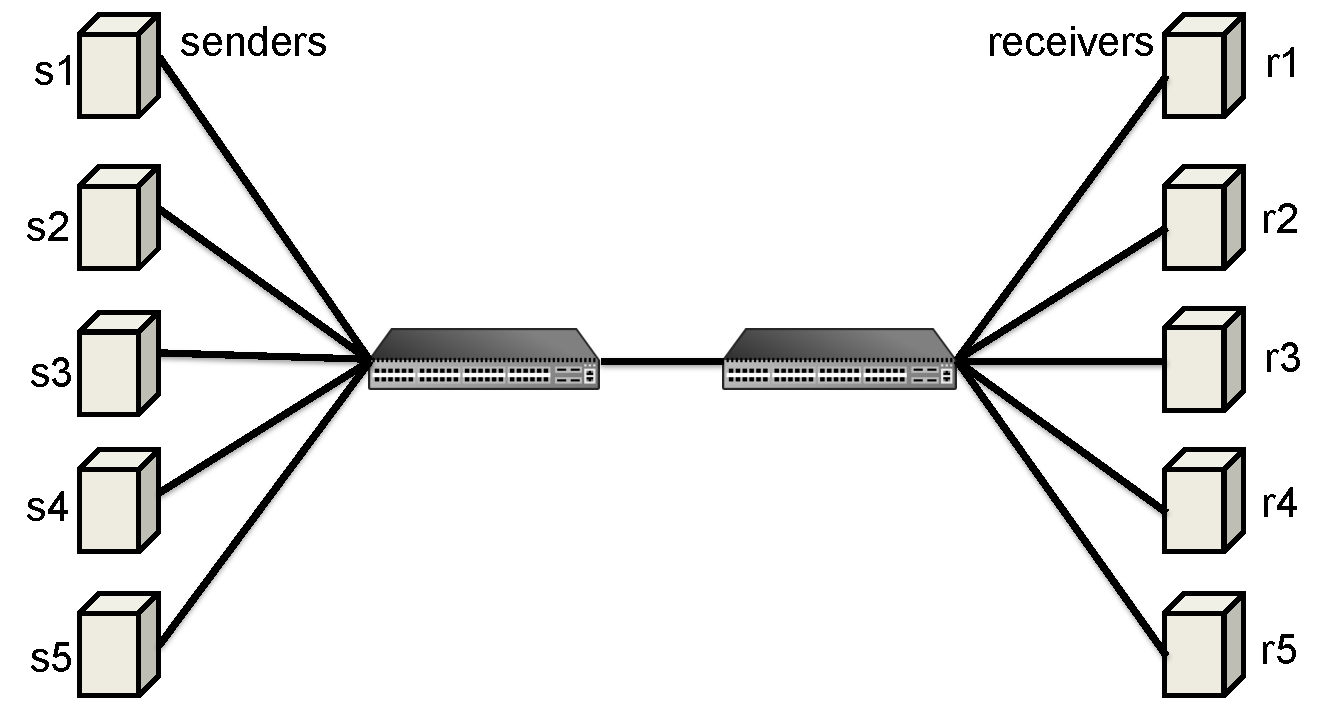
\includegraphics[width=0.7\textwidth]{figures/dumbbell_topology.pdf}
                \caption{Dumbbell topology.}
                \label{dumbbell_topology}
        \end{subfigure}
        \begin{subfigure}[b]{0.5\textwidth}
                \centering
                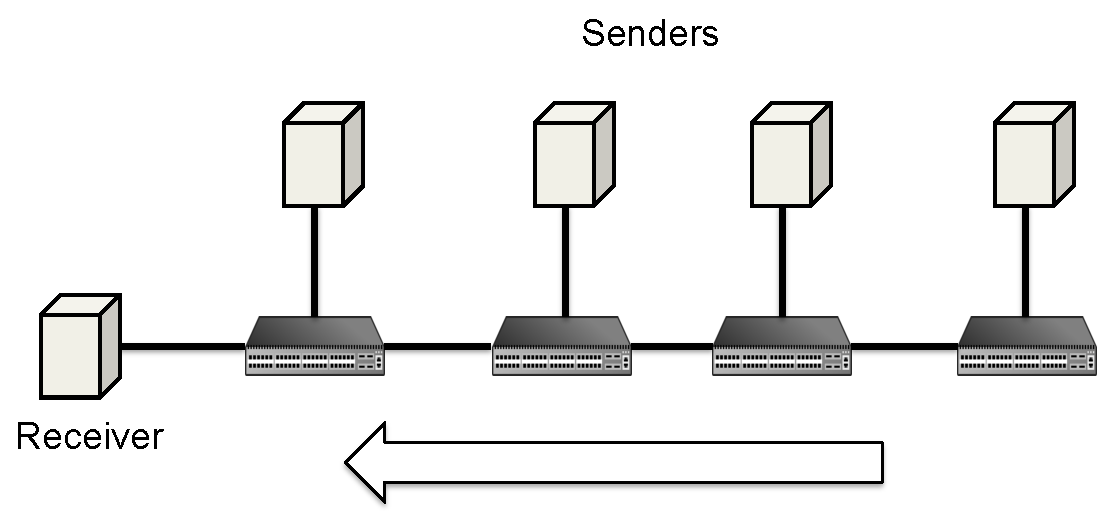
\includegraphics[width=0.7\textwidth]{figures/parkinglot_topology.pdf}
                \caption{Multi-hop, multi-bottleneck (parking lot) topology.}
                \label{parkinglot_topology}
        \end{subfigure}
        \caption{Experiment topologies.}
        \label{microbenchmarks_topology}
\end{figure}

%%%% topology %%%

\begin{figure}[!t]
        \centering
  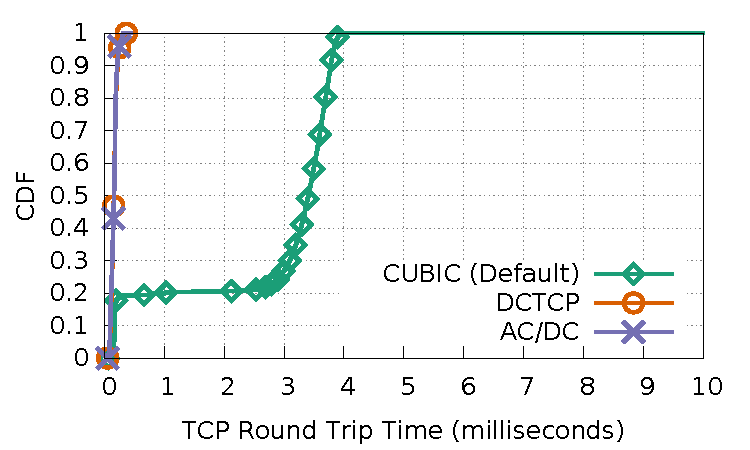
\includegraphics[width=0.45\textwidth]{figures/convergence/flowcontrolOFF_sockperf/convergence_test_sockperf.pdf}
        \caption{RTT of schemes on dumbbell topology.}
        \label{sockperf_convergence}
\end{figure}

We first evaluate \acdc{}'s performance using a set of microbenchmarks.
The microbenchmarks are conducted on topologies shown in Figure~\ref{microbenchmarks_topology}.

\tightparagraph{Canonical topologies}
We aim to understand the performance of our scheme on two simple topologies.
First, one long-lived flow is started per server pair ($s_i$ to $r_i$) in Figure~\ref{dumbbell_topology}. 
The average per-flow throughput of \acdc{}, DCTCP and CUBIC are all 1.98Gbps.
Figure~\ref{sockperf_convergence} is a CDF of the RTT
from the same test. Here, increases in RTT are caused by queueing delay in the switch.
~\acdc{} achieves comparable RTT with DCTCP and significantly outperforms CUBIC.

Second, each sender in Figure~\ref{parkinglot_topology} starts a long-lived
flow to the single receiver. Each flow traverses a different number of 
bottleneck links. CUBIC has an average per-flow throughput of 2.48Gbps with
a Jain's fairness index of 0.94, and
both DCTCP and \acdc{} obtain an average throughput of 2.45Gbps with a
fairness index of 0.99. 
The 50$^{th}$ and 99.9$^{th}$ percentile RTT for
\acdc{} (DCTCP, CUBIC) are 124$\mu$s (136$\mu$s, 3.3ms) and
279$\mu$s (301$\mu$s, 3.9ms), respectively.

%TCP-Bolt~\cite{stephens2014practical} and DCQCN~\cite{zhu2015congestion} found
%that Data Center Bridging (DCB) can have throughput unfairness and 
%increased queueing (bufferbloat) issues and such issues can be solved by utilizing
%ECN (like DCTCP). We anticipate our scheme can also work in DCB.

%%how close our RWND is to DCTCP's CWND
\begin{figure}[!t]
        \centering
        \begin{subfigure}[b]{0.225\textwidth}
                \centering
                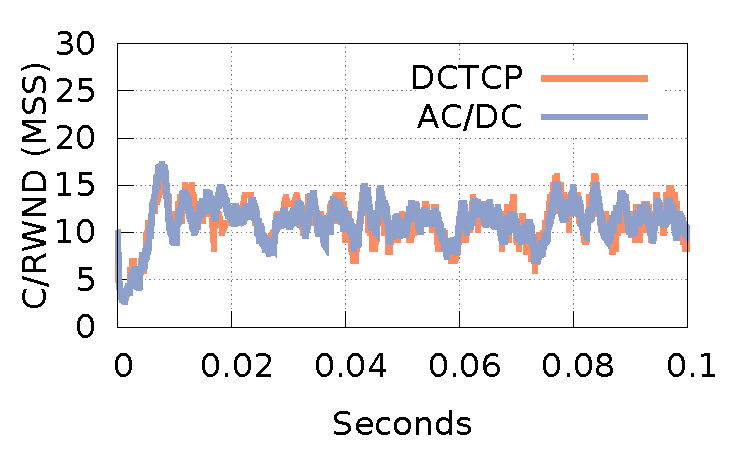
\includegraphics[width=\textwidth]{figures/cwnd_rwnd/newpara_refine/mtu1500_5flows_1/measure_cwnd_rwnd_gap_15k_5flows_0sec_100msec.pdf}
                \caption{First 100 ms of a flow.}
                \label{cwnd_rwnd_1500}
        \end{subfigure}
        \begin{subfigure}[b]{0.225\textwidth}
                \centering
                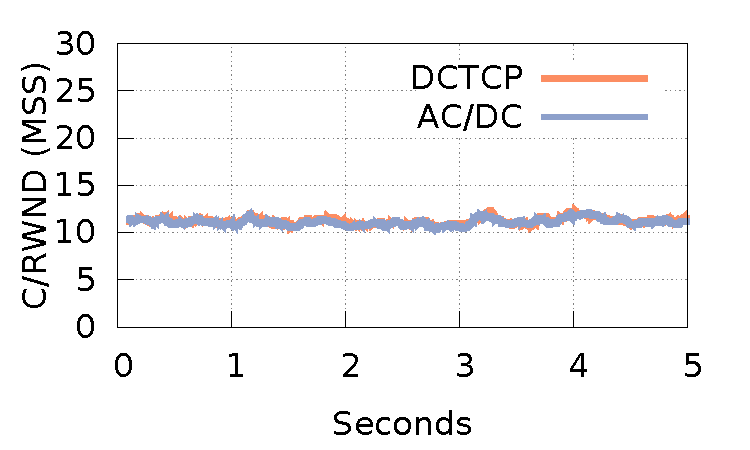
\includegraphics[width=\textwidth]{figures/cwnd_rwnd/moving-ave/measure_cwnd_rwnd_gap_15k_5flows_ave100.pdf}
                \caption{Moving average.}
                \label{cwnd_rwnd_1500_ave}
        \end{subfigure}

        \caption{~\acdc{}'s \rwnd{} tracks DCTCP's~\cwnd{}. MTU size = 1.5kB.}
        \label{compare_cwnd_rwnd}
\end{figure}



%%who limits TCP throughput, CWND or RWND? CUBIC
\begin{figure}[!t]
        \centering
        \begin{subfigure}[b]{0.225\textwidth}
                \centering
                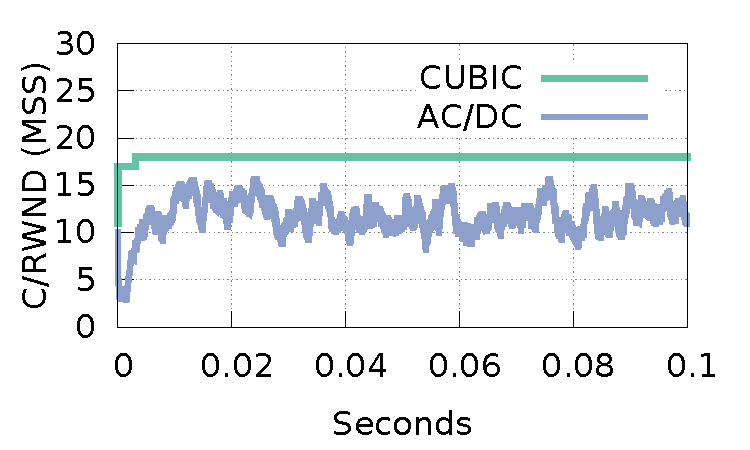
\includegraphics[width=\textwidth]{figures/cwnd_rwnd2/mtu1500_cubic/cubic_measure_cwnd_rwnd_gap_15k_5flows_0sec_100msec.pdf}
                \caption{Starting from 0 sec.}
                \label{who_limits_cwnd_rwnd_1500_0sec}
        \end{subfigure}
        \begin{subfigure}[b]{0.225\textwidth}
                \centering
                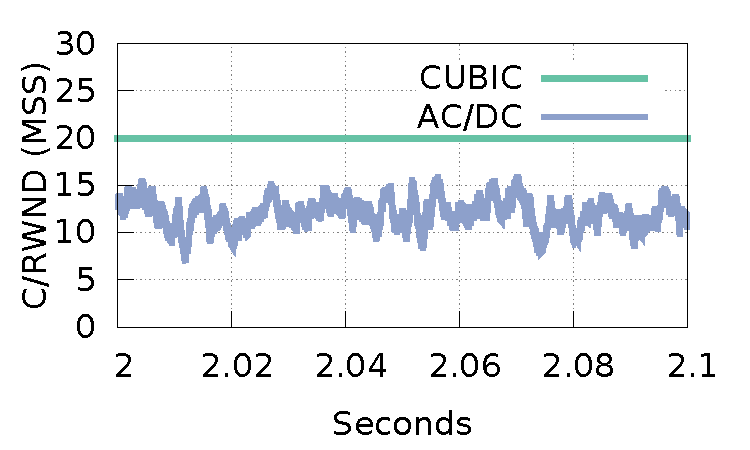
\includegraphics[width=\textwidth]{figures/cwnd_rwnd2/mtu1500_cubic/cubic_measure_cwnd_rwnd_gap_15k_5flows_2sec_100msec.pdf}
                \caption{Starting from 2 sec.}
                \label{who_limits_cwnd_rwnd_1500_2sec}
        \end{subfigure}
%        \begin{subfigure}[b]{0.225\textwidth}
%                \centering
%                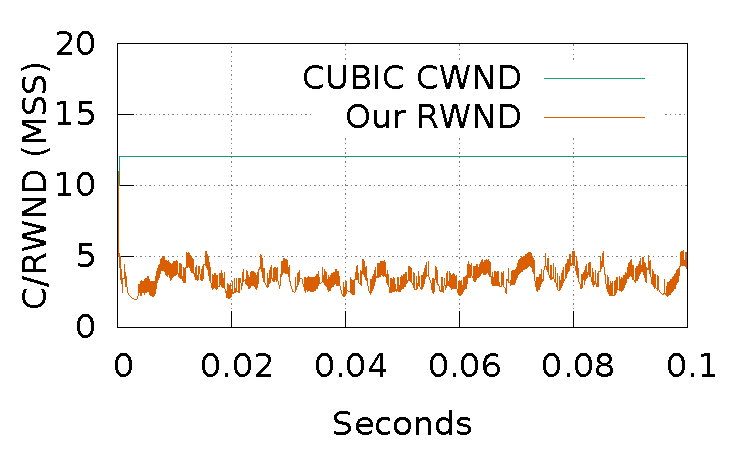
\includegraphics[width=\textwidth]{figures/cwnd_rwnd2/mtu9000_cubic/cubic_measure_cwnd_rwnd_gap_9k_5flows_0sec_100msec.pdf}
%                \caption{MTU9000: first 100 msec starting from second 0.}
%                \label{who_limits_cwnd_rwnd_9000_0sec}
%        \end{subfigure}
%        \begin{subfigure}[b]{0.225\textwidth}
%                \centering
%                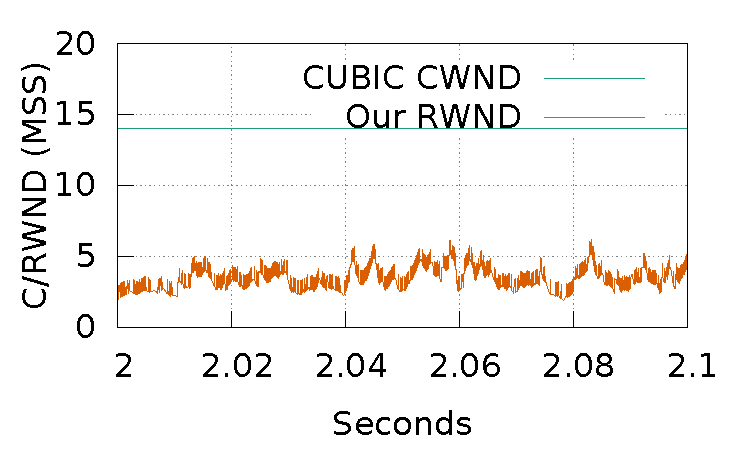
\includegraphics[width=\textwidth]{figures/cwnd_rwnd2/mtu9000_cubic/cubic_measure_cwnd_rwnd_gap_9k_5flows_2sec_100msec.pdf}
%                \caption{MTU9000: first 100 msec starting from second 2.}
%                \label{who_limits_cwnd_rwnd_9000_2sec}
%        \end{subfigure}
        \caption{Who limits TCP throughput when~\acdc{} is run with CUBIC? MTU = 1.5kB.}
        \label{who_limits_compare_cwnd_rwnd}
\end{figure}

\begin{figure}[t]
        \centering
  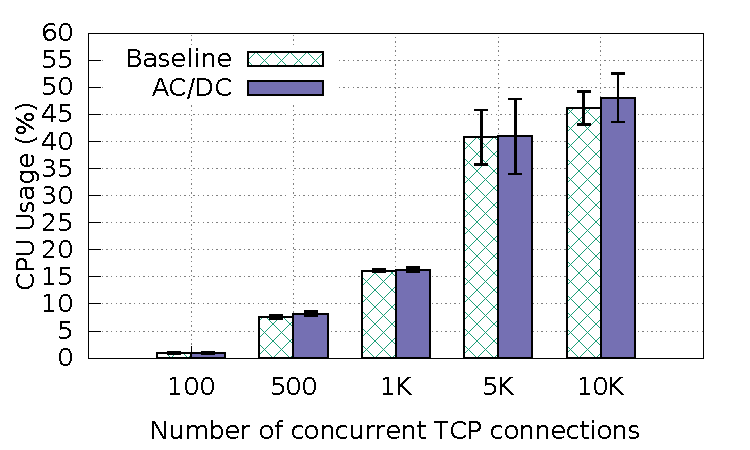
\includegraphics[width=0.45\textwidth]{figures/overhead/sender_15k_compare_cpu_witherrbar.pdf}
        \caption{CPU overhead: sender side (1.5kB MTU).}
        \label{cpu_overhead_sender_15k}
\end{figure}

\begin{figure}[t]
        \centering
  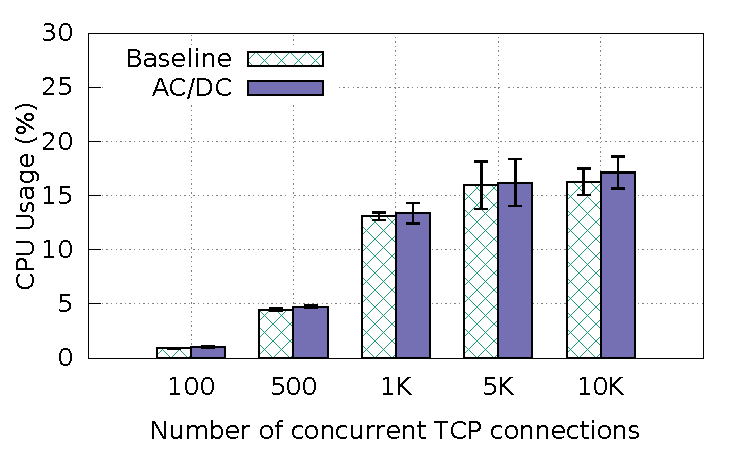
\includegraphics[width=0.45\textwidth]{figures/overhead/receiver_15k_compare_cpu_witherrbar.pdf}
        \caption{CPU overhead: receiver side (1.5kB MTU).}
        \label{cpu_overhead_receiver_15k}
\end{figure}

%%% other TCP variants %%%
\begin{table*}[!t]
\begin{center}
\begin{tabular}{ |c|c|c|c|c|c|c|c|c| }
 \hline
 \multirow{2}{*}{CC Variants} & \multicolumn{2}{|c|}{50$^{th}$ percentile RTT ($\mu$s)} & \multicolumn{2}{|c|}{99$^{th}$ percentile RTT ($\mu$s)} & \multicolumn{2}{|c|}{Avg Tput (Gbps)} & \multicolumn{2}{|c|}{Fairness Index}\\
 \cline{2-9}
       &  mtu=1.5kB & mtu=9kB & mtu=1.5kB & mtu=9kB & mtu=1.5kB & mtu=9kB & mtu=1.5kB & mtu=9kB\\
 \hline
 \hline
 CUBIC* &  3232     &   3448    &   3641     &  3865     &   1.89    & 1.98   &  0.85   &   0.98\\
 DCTCP* &  128      &   142    &   232    &   259    &   1.89    &   1.98  &  0.99    &   0.99\\
 \hline
 \hline
 CUBIC &   128     &   142    &    231    &   252    &   1.89    &  1.98   &  0.99    &  0.99 \\
 Reno  &   120     &   149    &    235    &   248    &   1.89    &  1.97   &  0.99    &  0.99 \\
DCTCP  &   129     &   149    &    232    &   266    &   1.88    &  1.98   &  0.99    &  0.99 \\
Illinois  &   134     &   152    &    215    &  262     &   1.89    &  1.97   &  0.99    &  0.99 \\
HighSpeed  &   119     &  147     &    224    &  252     &   1.88    & 1.97    &  0.99    & 0.99  \\
 Vegas  &   126     &   143    &    216    &    251   &   1.89    &  1.97   &  0.99    &  0.99 \\

 \hline

\end{tabular}
\caption{\acdc{} works with various kinds of congestion control variants.
        CUBIC*: CUBIC + standard OVS, switch WRED/ECN marking off.
        DCTCP*: DCTCP + standard OVS, switch WRED/ECN marking on.
        Others: different CCs + \acdc{}, switch WRED/ECN marking on.}
\label{other_cc_variants}
\end{center}
\end{table*}

\begin{figure}[t]
        \centering
  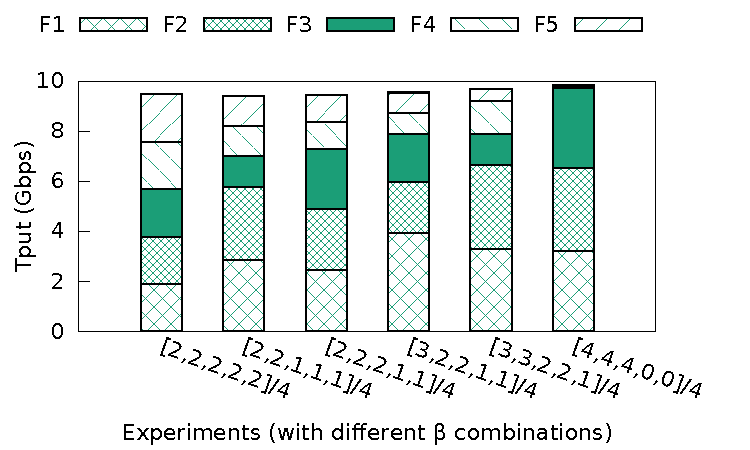
\includegraphics[width=0.45\textwidth]{figures/qos/qos_stacked.pdf}
        \caption{QoS-based CC.}
        \label{cc-qos}
\end{figure}

\tightparagraph{Tracking window sizes}
Next, we aim to understand how accurately~\acdc{} tracks DCTCP's performance at a finer level. The host's TCP
stack is set to DCTCP and our scheme runs in the vSwitch.
We repeat the experiment in Figure~\ref{dumbbell_topology} and measure the~\rwnd{} calculated by~\acdc{}. Instead
of over-writing the~\rwnd{} value in the ACKs, we simply log the value to a file. Thus, congestion is enforced by DCTCP
and we can capture DCTCP's~\cwnd{} by using {\tt tcpprobe}~\cite{tcp-probe}. We align the~\rwnd{} and~\cwnd{} values by timestamps and sequence
numbers and show a timeseries in Figure~\ref{compare_cwnd_rwnd}. Figure~\ref{cwnd_rwnd_1500} shows both windows for the
first 100 ms of a flow and shows that~\acdc{}'s calculated window closely tracks DCTCP's. Figure~\ref{cwnd_rwnd_1500_ave} 
shows the windows over a 100ms moving average are also similar. This suggests that it is easy to accurately recreate congestion
control in the vSwitch. Note we obtained results for 9kB MTU that were similar.

We were also interested to see how often~\acdc{}'s congestion window takes effect. We rerun the experiment, but set
the host TCP stack to CUBIC. The~\rwnd{} computed by~\acdc{} is both written into the ACK and logged to a file. We again
use {\tt tcpprobe} to measure CUBIC's~\cwnd{}. Figure~\ref{who_limits_compare_cwnd_rwnd} is a timeseries (one graph from the
start of the experiment and one graph 2 seconds in) that shows~\acdc{}'s
congestion control algorithm is indeed the limiting factor.
In the absence of loss or ECN markings, traditional TCP stacks do not severely reduce~\cwnd{} and thus
\acdc{}'s~\rwnd{} becomes the main enforcer of a flow's congestion control. Because DCTCP 
is effective at reducing loss and~\acdc{} hides ECN feedback from the host TCP stack,
~\acdc{}'s enforcement is applied often.
%As before, 9kB MTU results showed similar trends.

%
%\begin{figure}[!htb]
%        \centering
%  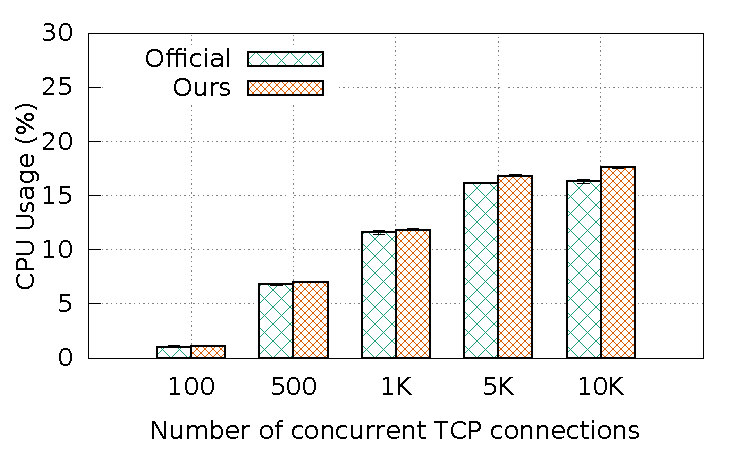
\includegraphics[width=0.45\textwidth]{figures/overhead/sender_9k_compare_cpu_witherrbar.pdf}
%        \caption{CPU overhead: sender side (9K MTU). The 10G NIC is saturated when there are more than 1K TCP connections.
%		CPU usage refers to the CPU usage of the whole server (12 Intel(R) Xeon(R) CPU E5649@2.53GHz processors)
%                measured by ``sar (sysstat)''.}
%        \label{cpu_overhead_sender_9k}
%\end{figure}
%
%\begin{figure}[!htb]
%        \centering
%  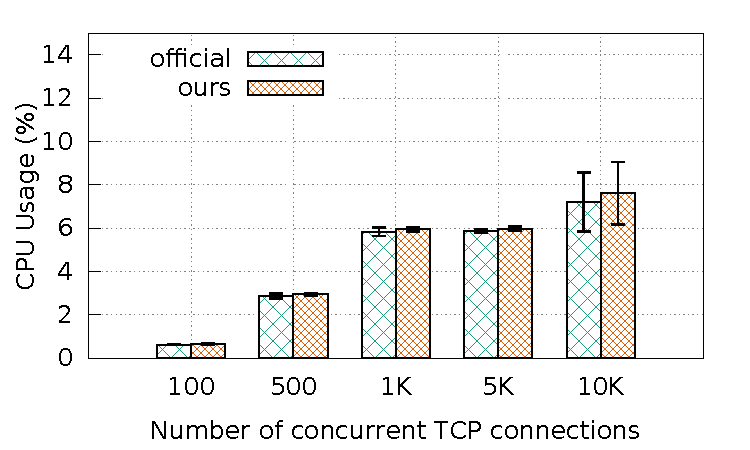
\includegraphics[width=0.45\textwidth]{figures/overhead/receiver_9k_compare_cpu_witherrbar.pdf}
%        \caption{CPU overhead: receiver side (9K MTU). The 10G NIC is saturated when there are more than 1K TCP connections.
%		CPU usage refers to the CPU usage of the whole server (12 Intel(R) Xeon(R) CPU E5649@2.53GHz processors)
%                measured by ``sar (sysstat)''}
%        \label{cpu_overhead_receiver_9k}
%\end{figure}
%

\tightparagraph{CPU overhead}
We measure the CPU overhead of~\acdc{} by connecting two servers to a single switch. 
Multiple simultaneous TCP flows are started from one server to the other and the total CPU utilization
is measured on the sender and receiver using {\tt sar}. Each flow is given time to perform the TCP handshake
and when all are connected, each TCP client sends with a demand of 10 Mbps by sending 128 kB bursts every 100 milliseconds (so 1,000 connections saturate the 10 Gbps link). 
The CPU overhead of~\acdc{} compared to the CPU overhead of baseline (\ie{}, just OVS) 
is shown for the sender in Figure~\ref{cpu_overhead_sender_15k}
 and the receiver in Figure~\ref{cpu_overhead_receiver_15k}. Even when scaling to 
10,000 connections, 
the CPU overhead of our scheme is less than 4\%. 
Note experiments with 9kB MTU have similar trends,
but we show the 1.5kB MTU case because smaller MTU sizes incur higher overhead.


%%%convergence %%%
\begin{figure*}[t]
        \centering
        \begin{subfigure}[b]{0.33\textwidth}
                \centering
                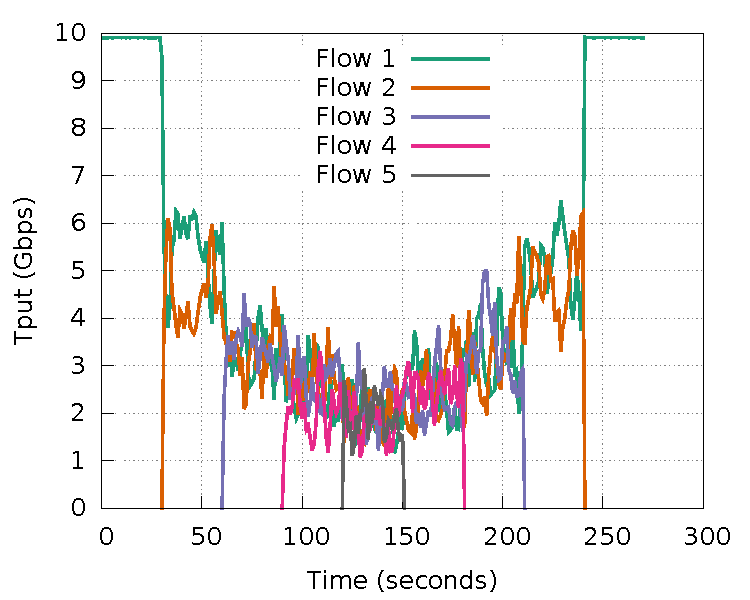
\includegraphics[width=\textwidth]{figures/convergence/flowcontrolOFF/tcp_flowcontrolOFF_convergence.pdf}
                \caption{CUBIC convergence test.}
                \label{cubic_convergence}
        \end{subfigure}
        \begin{subfigure}[b]{0.33\textwidth}
                \centering
                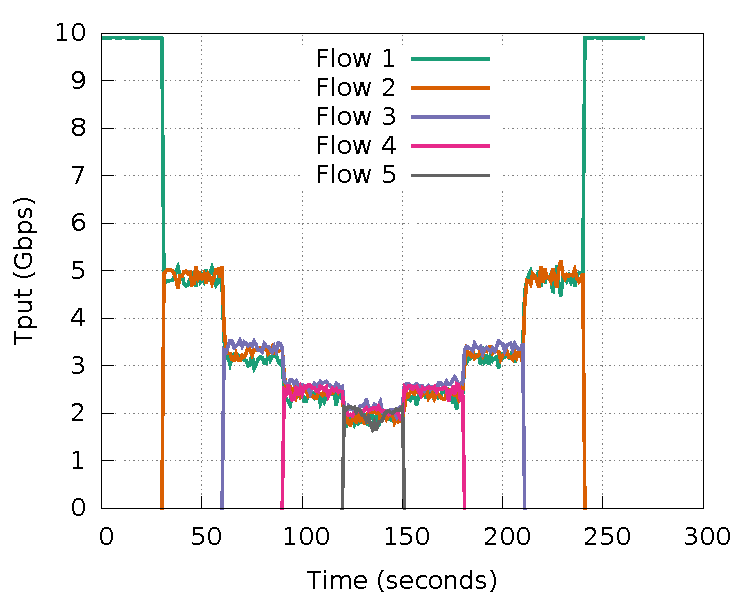
\includegraphics[width=\textwidth]{figures/convergence/flowcontrolOFF/dctcp_flowcontrolOFF_convergence.pdf}
                \caption{DCTCP convergence test.}
                \label{dctcp_convergence}
        \end{subfigure}
        \begin{subfigure}[b]{0.33\textwidth}
                \centering
                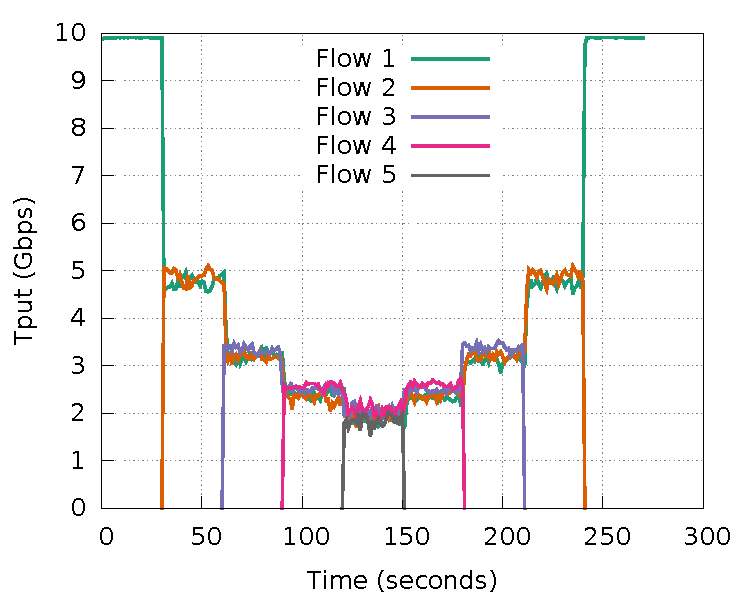
\includegraphics[width=\textwidth]{figures/convergence/flowcontrolOFF/ovsdctcp_flowcontrolOFF_convergence.pdf}
                \caption{\acdc{} convergence test.}
                \label{ovsdctcp_convergence}
        \end{subfigure}
        \caption{Convergence tests.}
        \label{convergence_test}
\end{figure*}


\tightparagraph{~\acdc{} flexibility}~\acdc{} aims to provide a degree of control and flexibility over tenant TCP stacks. 
We consider two cases.
First,~\acdc{} should work effectively, regardless of the tenant TCP stack.
Table~\ref{other_cc_variants} shows the performance of our scheme when various TCP congestion control algorithms
are configured on the host. Data is collected over 10 runs lasting 20 seconds each on the dumbbell topology (Figure~\ref{dumbbell_topology}). 
The first two rows of the table, CUBIC* and DCTCP*, show the performance of each stack with an 
unmodified OVS. The next six rows show the performance of a given host stack with~\acdc{} running DCTCP in OVS.
The table shows~\acdc{} can effectively track the performance of DCTCP, meaning 
it is compatible with popular delay-based (Vegas) and loss-based (Reno, CUBIC, etc) stacks.

Second,~\acdc{} enables an administrator to assign different 
congestion control algorithms on a per-flow basis. 
%For example, congestion control algorithms shown to optimize WAN performance, 
%such as Compound TCP~\cite{tan2006compound}, can be employed on front-end
%web server traffic, while DCTCP can be used for intra-DC back-end traffic.
For example,~\acdc{} can provide the flexibility to implement QoS through differentiated congestion control. 
We fix the host TCP stack to CUBIC and alter~\acdc{}'s congestion control for each flow
by setting the $\beta$ value (in Equation~\ref{eqn:cc-qos}) for each flow in the dumbbell topology. 
Figure~\ref{cc-qos} shows the throughput achieved by each flow, 
along with its $\beta$ setting.~\acdc{} is 
able to provide relative bandwidth allocation to each flow based on $\beta$. 
Flows with the same $\beta$ value get similar throughputs and flows with higher $\beta$ values 
obtain higher throughput.
The latencies (not shown) remain consistent with
previous results.


%%%coexistence %%%
\begin{figure}[!t]
        \centering
        \begin{subfigure}[b]{0.225\textwidth}
                \centering
                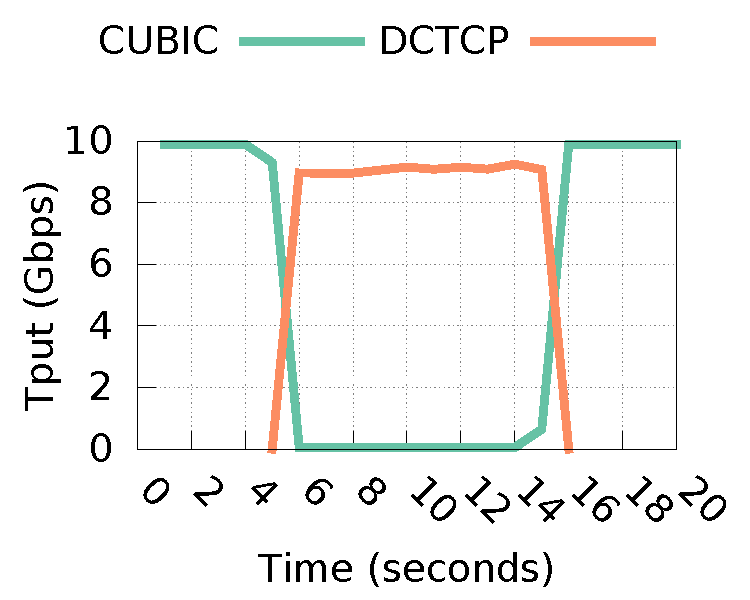
\includegraphics[width=\textwidth]{figures/micro2flows/coexitence/cubic_dctcp_coexistence_official.pdf}
                \caption{Default.}
                \label{coexistence_tput_ovs}
        \end{subfigure}
        \begin{subfigure}[b]{0.225\textwidth}
                \centering
                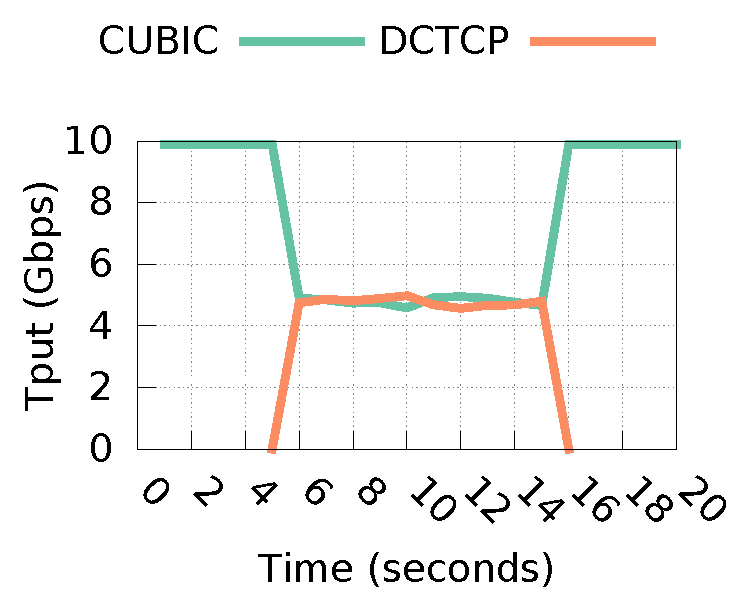
\includegraphics[width=\textwidth]{figures/micro2flows/coexitence/cubic_dctcp_coexistence_acdctcp.pdf}
                \caption{\acdc{}.}
                \label{coexistence_tput_ovsdctcp}
        \end{subfigure}
        \caption{(a) CUBIC gets little throughput when competing with DCTCP.
		 (b) With \acdc{}, CUBIC and DCTCP flows get fair share.}
        \label{coexistence_tput}
\end{figure}

\begin{figure}[!t]
        \centering
  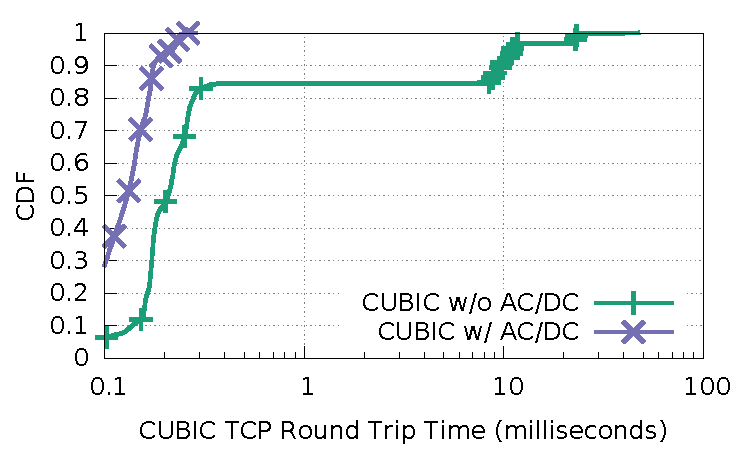
\includegraphics[width=0.45\textwidth]{figures/micro2flows/coexitence/sockperf_and_droprate/coexistence_sockperf.pdf}
        \caption{CUBIC experiences high RTT when competing with DCTCP.~\acdc{} fixes this issue.}
        \label{coexistence_sockperf_droprate}
\end{figure}

\begin{figure}[!t]
        \centering
%        \begin{subfigure}[b]{0.24\textwidth}
%                \centering
%                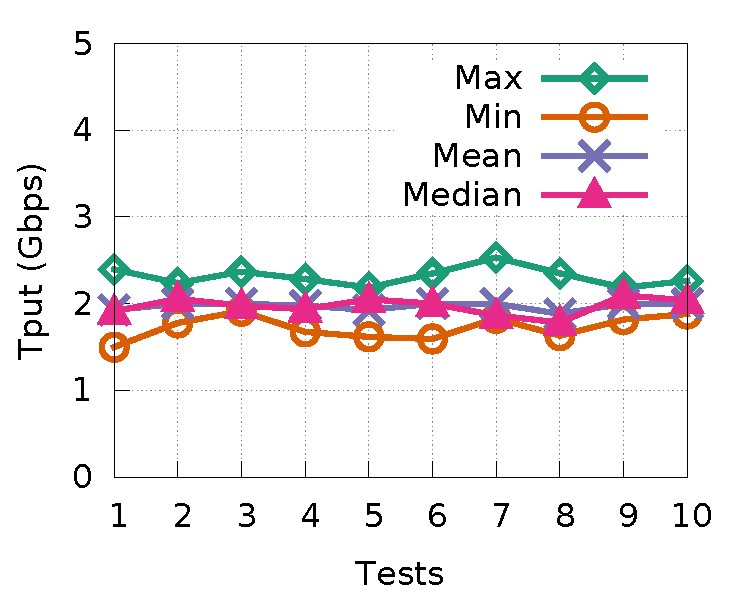
\includegraphics[width=\textwidth]{figures/tput_fairness/default_all_cubic_tput.pdf}
%                \caption{All CUBIC.}
%                \label{fairness_all_cubic}
%        \end{subfigure}
%        \begin{subfigure}[b]{0.24\textwidth}
%                \centering
%                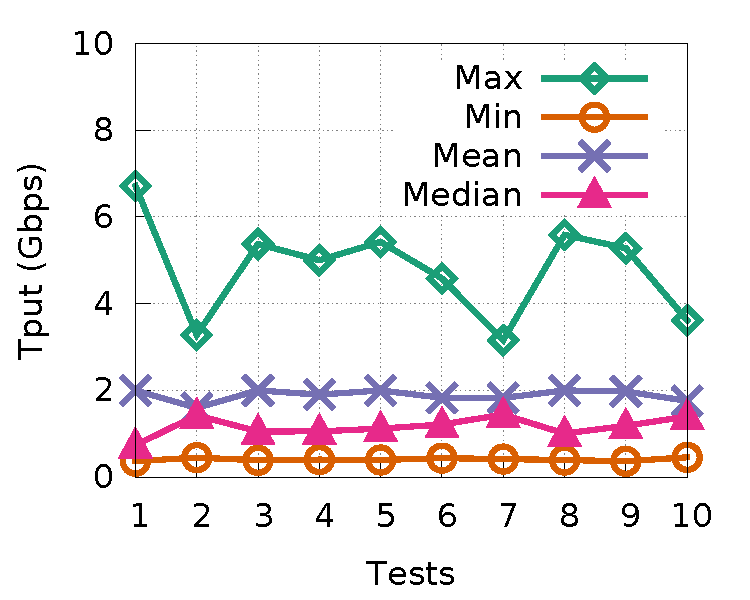
\includegraphics[width=\textwidth]{figures/tput_fairness/default_5CC_tput.pdf}
%                \caption{5 different CCs.}
%                \label{fairness_5CC}
%        \end{subfigure}
        \begin{subfigure}[b]{0.225\textwidth}
                \centering
                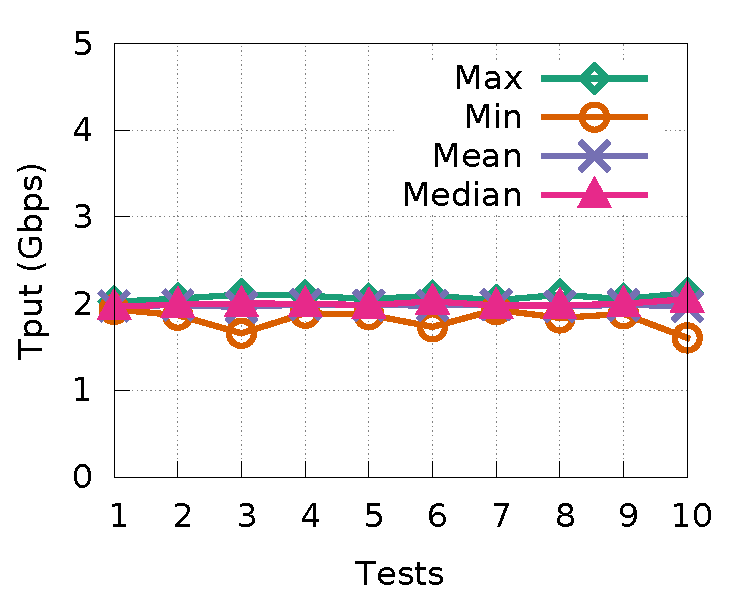
\includegraphics[width=\textwidth]{figures/tput_fairness/ecn_all_dctcp_tput.pdf}
                \caption{All DCTCP.}
                \label{fairness_5CC_with_dctcp}
        \end{subfigure}
        \begin{subfigure}[b]{0.225\textwidth}
                \centering
                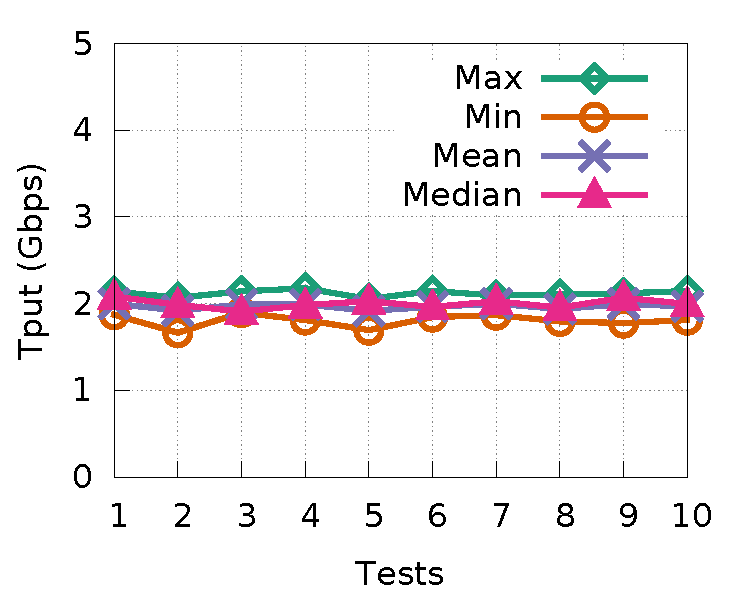
\includegraphics[width=\textwidth]{figures/tput_fairness/liquid_5CC_tput.pdf}
                \caption{5 different CCs with \acdc{}.}
                \label{fairness_5CC_with_ours}
        \end{subfigure}
	\caption{\acdc{} improves TCP fairness.} 
 	\label{tput_fairness_coexistence}
\end{figure}	


\tightparagraph{Fairness}
Three different experiments are used to demonstrate fairness. First, we aim to show~\acdc{} can mimic DCTCP's 
behavior in converging to fair throughputs. We repeat the experiment originally performed 
by Alizadeh~\cite{alizadeh2011data} and Judd~\cite{judd2015nsdi} by 
adding a new flow every 30 seconds on a bottleneck link, and then reverse the process. 
The result is shown in Figure~\ref{convergence_test}.
Figure~\ref{cubic_convergence} shows CUBIC's problems converging to fair allocations.
Figures~\ref{dctcp_convergence}
and~\ref{ovsdctcp_convergence} show DCTCP's and~\acdc{}'s performance, respectively.~\acdc{} tracks DCTCP's behavior.
CUBIC's drop rate is 0.17\% while DCTCP's and \acdc{}'s is 0\%. 
%Note that as mentioned in~\cite{judd2015nsdi}, CUBIC's 
%performance can be improved by manually altering the socket buffer size, 
%but let applications sizing it in practice is hard. DCTCP, and thus
%our scheme, do not need this optimization, 
%thus demonstrating one additional benefit of our approach.

The second experiment is also repeated from Judd's paper~\cite{judd2015nsdi}. 
ECN-capable and non-ECN-capable flows do not coexist well because switches
drop non-ECN packets when the queue length is larger than the predefined
marking threshold. Figure~\ref{coexistence_tput_ovs}
shows the throughput of CUBIC suffers when CUBIC (with no ECN) and DCTCP (with ECN) traverse the same bottleneck link.
Figure~\ref{coexistence_tput_ovsdctcp} shows this problem is alleviated with~\acdc{}
because it forces all flows 
to become ECN-capable when they enter fabric.
Figure~\ref{coexistence_sockperf_droprate} shows CUBIC's RTT is extremely high
in the first case because switches drop non-ECN packets (the loss rate is 0.18\%) and thus
there is a significant number of retransmissions. However, implementing~\acdc{} eliminates 
this issue and reduces latency.
%\emph{\acdc{} makes low latency possible in production data center networks where
%incremental deployment is the norm and transport diversity must be supported}.

The last experiment examines the impact of having multiple TCP stacks on the same fabric. 
Five flows with different congestion control algorithms (CUBIC, Illinois, HighSpeed, New Reno and Vegas) are started
on the dumbbell topology. This is the same experiment as in Figure~\ref{tput_unfair}.
Figure~\ref{fairness_5CC_with_dctcp} shows what happens if all
flows are configured to use DCTCP and Figure~\ref{fairness_5CC_with_ours} shows when
the five different stacks traverse~\acdc{}. We can see~\acdc{} closely tracks the ideal case of
all flows using DCTCP, and~\acdc{} and DCTCP provide better fairness than all CUBIC (Figure~\ref{unfairness_all_cubic}).
%The median and 99.9\% TCP RTTs for all CUBIC, 5 different CCs, 5 different CCs with
%our logic and all DCTCP are: 3.5 ms, 3.9 ms; 3.4 ms, 4.0 ms; 146 $\mu$s, 306 $\mu$s;
%147 $\mu$s, 317 $\mu$s. Both~\acdc{} and DCTCP obtain a Jain's fairness index greater than 0.99.


\iffalse
\tightparagraph{Different MTU sizes}
We set MTU size to 1500 bytes and run the tests on the dumbbell topology (Figure~\ref{dumbbell_topology})
with 5 flows competing for
a 10G bottleneck link. \acdc{} gets 1.87Gbps average flow throughput. DCTCP gets 1.88Gbps average flow throughput. 
Both have a Jain's fairness index greater than 0.99. TCP CUBIC gets 1.89 average flow throughput and a fairness index of 0.85.
The 50$^{th}$ and 99.9$^{th}$ percentile TCP RTT for \acdc{} (DCTCP, CUBIC) are 139$\mu$s (136$\mu$s, 3.2ms) and
359$\mu$s (342$\mu$s, 3.7ms), respectively.
~\eric{KEQIANG: please look at this paragraph and see how it fits in the
"Canonical Topologies" paragraph. Our numbers should be consistent. We can 
remove this paragraph afterwards.}
\fi
